


\documentclass[multi,crop,tikz,border=0pt,12pt]{standalone}

\usepackage{latexsym,mathtools}



\begin{document}




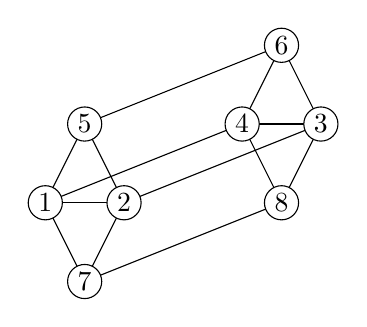
\begin{tikzpicture}[scale=0.5]
    % Define points of the cuboid
    \coordinate (1) at (-2,0);
    \coordinate (2) at (0,0);
    \coordinate (5) at (-1,2);
    \coordinate (7) at (-1,-2);

    \coordinate (4) at (3,2);
    \coordinate (3) at (5,2);
    \coordinate (6) at (4,4);
    \coordinate (8) at (4,0);

    % Draw edges
    \draw (1) -- (5) -- (2) -- (7) -- cycle;
    \draw (4) -- (6) -- (3) -- (8) -- cycle;
    \draw (1) -- (2);
    \draw (3) -- (4);
    \draw (5) -- (6);
    \draw (1) -- (4);
    \draw (2) -- (3);
    \draw (7) -- (8);

    % Label vertices
    \foreach \i in {1,...,8} {
        \node[fill=white, circle, draw, inner sep=1.5pt] at (\i) {\i};
    }
\end{tikzpicture}

\end{document}
